\documentclass{bioinfo}
\copyrightyear{2005}
\pubyear{2005}

\begin{document}
\firstpage{1}

\title[short Title]{Seeq: a library for inexact DNA sequence matching}
\author[Zorita \textit{et~al}]{Eduard Zorita\,$^{1,2}$ and Guillaume J. Filion\,$^{1,2}$\footnote{to whom correspondence should be addressed}}
\address{$^{1}$Genome Architecture, Gene Regulation, Stem Cells and
  Cancer Programme, Centre for Genomic Regulation (CRG), Dr. Aiguader
  88, 08003 Barcelona, Spain\\
$^{2}$Universitat Pompeu Fabra (UPF), 08002 Barcelona, Spain}

\history{Received on XXXXX; revised on XXXXX; accepted on XXXXX}

\editor{Associate Editor: XXXXXXX}

\maketitle

\begin{abstract}

\section{Motivation:}
Searching specific sequences over DNA reads is an elemental procedure
of biological data analysis. Experimental DNA samples have usually
been engineered to contain pattern sequences at the positions where
operations such as adaptor removal, sequence trimming or barcode
extraction have to be performed. The experimental data contain errors
that must be tolerated in order to identify these patterns at their
correct positions. This process is straightforward in data produced by
second generation sequencing machines, in which the error rates lie
below 2\%. Short sequences with small error tolerance suffice to
identify the patterns accurately in these circumstances. However,
third generation sequencing technologies promise longer reads with
error rates around 15\%. Consequently, this opens a new scenario in
which both the pattern length and the relative error tolerance will
have to be dramatically increased.
\section{Results:}
In this paper we present seeq, an inexact pattern matching algorithm
optimized for DNA sequence matching with almost constant running
time. We benchmark seeq against the most widely used algorithms for
inexact pattern matching. The results show that seeq scales better and
becomes significantly faster as the error rate increases.
\section{Availability:}
Seeq is available in three forms: Linux software, C Library and Python
module. The source code and the C/Python libraries are available for
download at
\href{http://github.com/ezorita/seeq}{http://github.com/ezorita/seeq}.
\section{Contact:} \href{guillaume.filion@gmail.com}{guillaume.filion@gmail.com}
\end{abstract}

\section{Introduction}

Inexact string matching is an old problem that dates back to the
sixties with the definition of the edit distance \citep{Lev65}. The
first algorithms used to solve this problem were based on dynamic
programming \citep{NW70}. Although the algorithms were not very
efficient, they are still widely used to align biological sequences
due to their simplicity and flexibility. Later on, more sophisticated
algorithms derived from the Boyer-Moore search method \citep{BM77}
were designed to search patterns on long strings allowing
differences. Such algorithms are much faster than the dynamic
programming approach because they do not compute all the relative
distances. Instead, the pattern is pre-processed to design a search
strategy which skips parts of the text that do not contain any
match. The jumping strategy is very efficient for perfect matches or
small edit distances because the non-matching condition is inferred
with only a few comparisons. In this scenario, the number of
operations per input character is ridiculously small given that large
areas of the text are never processed. However, other scenarios are
not so favorable for this technique. For instance, if the proposed
pattern matches in almost any text position, the performance degrades
severely since the algorithm will not be able to jump so
often. Besides, for high mismatch ratios the search strategy becomes
complex and requires more comparisons to determine a non-matching
condition, specially when the alphabet is as small as in the task of
matching DNA sequences.

Sequencing data produced by the Illumina platform \citep{Mar05}
typically has 1-2\% error rate mainly consisting of substitutions
\citep{Doh08}. Therefore one expects to find all the matching strings
within a small edit distance relative to the original pattern
length. Moreover, if such patterns are produced artificially
(e.g. sequencing adaptors or barcodes), it is reliable to use short 
sequences that are not present in the target genome. On the other
side, the PacBio platform produces reads two orders of magnitude
longer than Illumina, but at the expense of a much higher error rate
(15\%) consisting principally of insertions and deletions
\citep{Eid09}. This high error rate dramatically increases the false
positive rate unless the pattern sequence is extended
accordingly. This brings us to a new scenario with unusually long
patterns and edit distances that lie on the same order of magnitude.

In this article we present \emph{seeq}, an algorithm based on a
deterministic finite automaton (DFA) structure. The automaton is built
as the input text is processed and has been optimized for DNA sequence
matching. We benchmark seeq against other widely used inexact string
matching software. The results show that seeq scales better and
becomes significantly faster as the error rate increases.

\begin{methods}
\section{Methods}

The algorithm proposed is the DFA representation of a dynamic
programming algorithm. The goal is to find the occurrences of a
pattern $P$ in a text $T$ that are $k$-differences or less. The
lengths of $P$ and $T$ are $m$ and $n$, respectively. The score matrix
$\mathbf{C} \in \mathbb{N}^{m\times n}$ is initialized so as that any
text position is a potential alignment start, i.e. $\mathbf{C}(0,j)=0$
and $\mathbf{C}(i,0) = i$. After the initialization, the score matrix
is computed and filled column-wise. Note that the standard dynamic
programming update process can be represented as
$\mathbf{c}_j=f(\mathbf{c}_{j-1},T_j)$. In effect, the value of the 
$j$-th column $\mathbf{c}_{j}$ is a deterministic transition that only
depends on $\mathbf{c}_{j-1}$ and the character $T_j$. We take
advantage of this property to build a deterministic automata in which
the different states represent the set of non-equivalent alignment
columns and the transitions between states are dictated by the input
characters.

To make the alignment algorithm efficient, only the significant
($\mathbf{C}(i,j) \le k$) parts of the column are computed. The DFA
states $S$ have a vector representation
$\mathbf{s} = \mbox{dif}(\mathbf{c}_j)$ generated by differentially
encoding the $j$-th column values as 
$\mathbf{s}(i)=\mathbf{C}(i+1,j)-\mathbf{C}(i,j)+1$ for
$i=0\ldots m-1$. This is done for two reasons: (i) the alphabet of
$\mathbf{s}$ is small \{0,1,2\}, therefore the alignment columns can be
efficiently stored in a ternary trie, and (ii) the inverse process to
recompute the original column ($\mathbf{c}_j=\mbox{undif}(\mathbf{s})$)
is performed without further information, provided that $\mathbf{C}(0,j)=0$. 

\begin{figure}[!tpb]
%\centerline{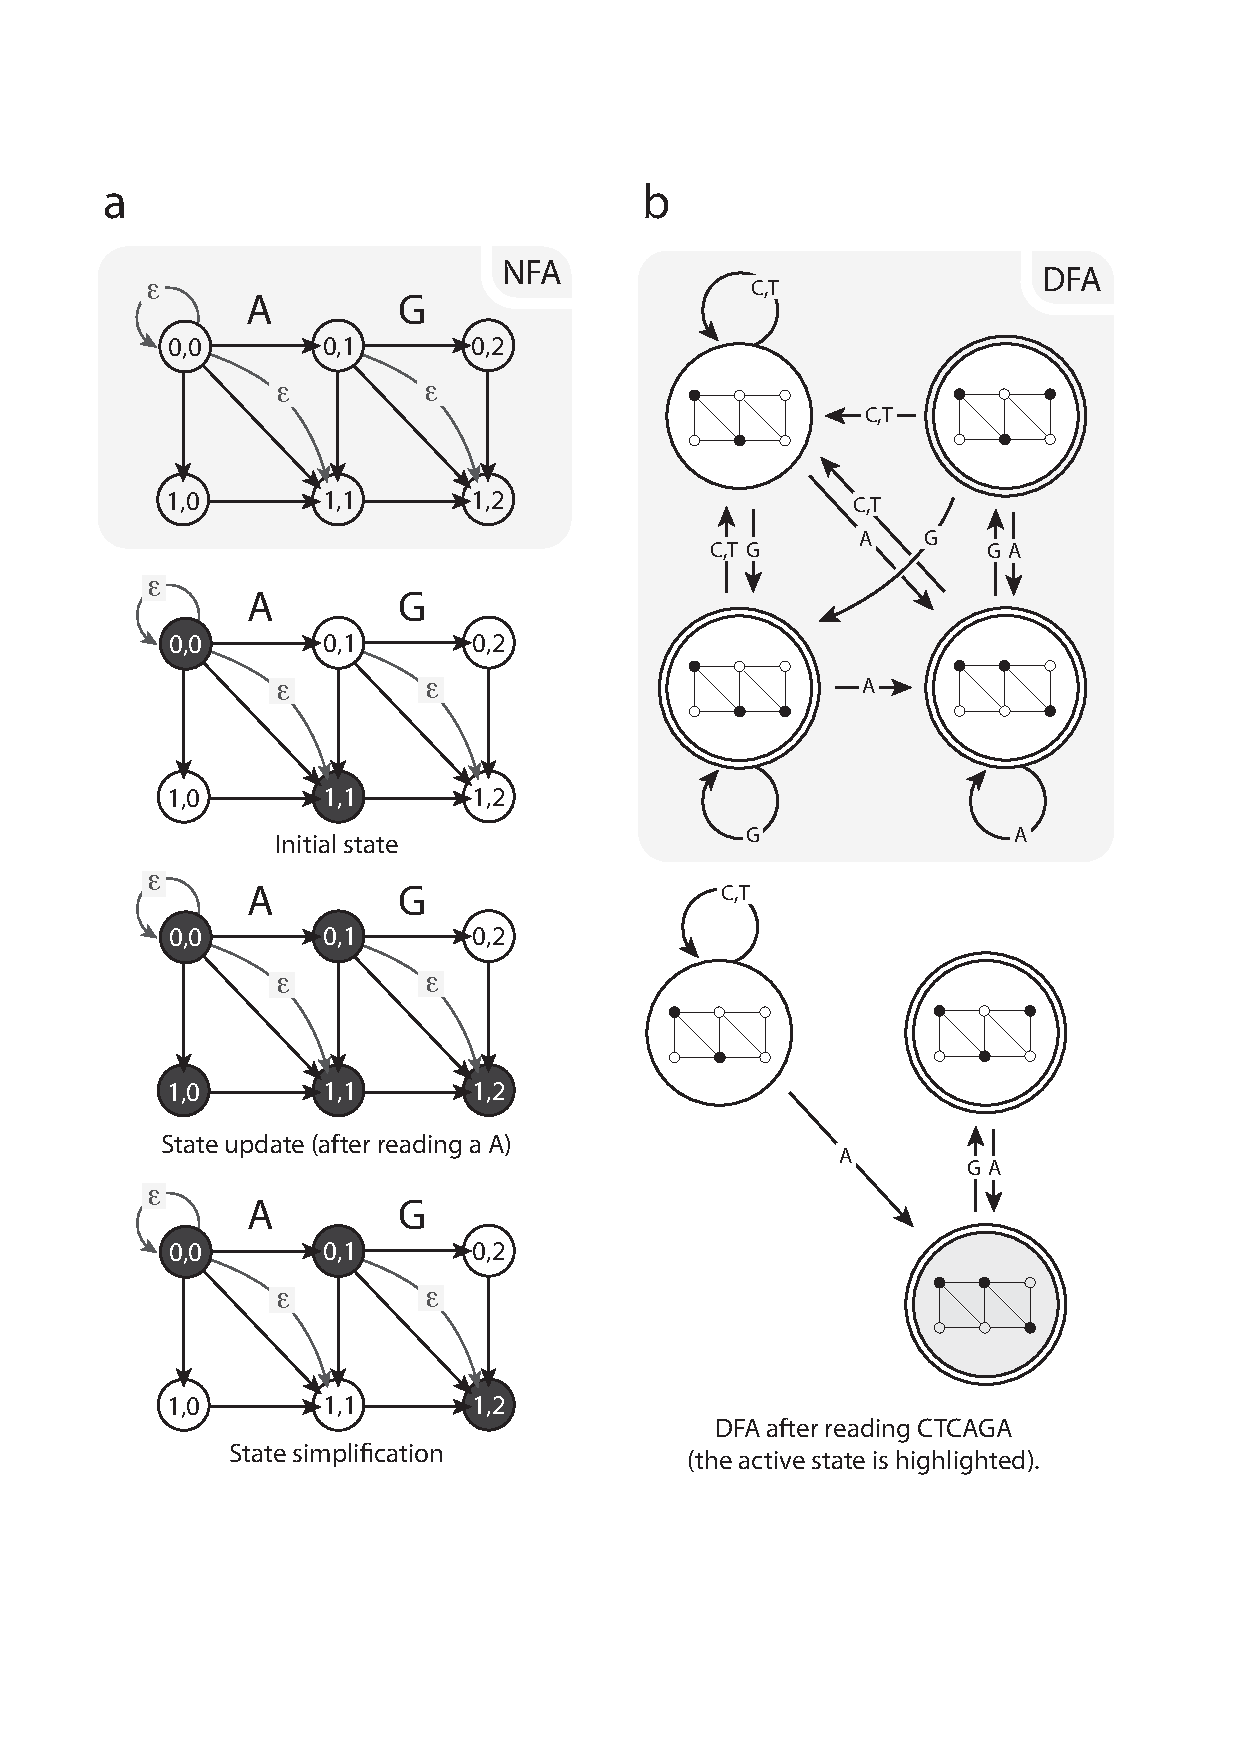
\includegraphics[scale=0.5]{fig_methods.pdf}}
\caption{}\label{matrix}
\end{figure}

The DFA construction process is illustrated in Figure. X. The
dynamic programming algorithm starts at the DFA state
$S = S_0$. For any input character $T_j$, being $S$
the active DFA state, the algorithm recursively proceeds as follows:
\begin{itemize}
\item If $S$ has an outgoing path (to $S_q$) with
label $T_j$, then $S = S_q$.
\item Otherwise, the vector $\mathbf{s}_j$ is computed as
$\mathbf{s}_j=\mbox{dif}(f(\mbox{undif}(\mathbf{s}), T_j))$.
If a state represented by $\mathbf{s}_j$ already exists ($S_q$), $S$
is connected to such state with a path labeled $T_j$ and $S = S_q$. On
the other hand, if $\mathbf{s}_j$ does not exist, a new DFA state
$S_j$ is created and both nodes are connected in the same
way, then $S = S_j$.
\end{itemize}
After several steps, the DFA graph is densely connected and the
complexity of the algorithm boils down to direct DFA state
transitions.

\end{methods}

\section{Results}

We have benchmarked seeq against two competitive inexact string
matching algorithms: agrep \citep{Wu92} and nr-grep \citep{Nav01}. We
used two real sequencing datasets for benchmarking. Both datasets contain
10 million reads but differ in read length. Dataset 1 consists random
Drosophila genome reads of length 100. Dataset 2 reads are 50
nucleotides long, from which the first 30 nucleotides are constant and
the last 20 are random (barcodes). The software were set to match
random patterns ranging from 5 to 50 nucleotides with a random error
tolerance up to 40\%. We would like to point out that agrep limits the
number of differences to 8, therefore the comparison shown here is
only fair between seeq and nr-grep.

Figure \ref{fig:results} shows the running time of each execution as
a function of the relative error tolerace ($k/m$). For low error
rates, both agrep and nr-grep perform better than seeq, with a maximum
5-fold advantage when $k=1$ and $m > 25$. On the other hand, seeq is
up to two orders of magnitude faster than nr-grep and one order of
magnitude faster than agrep for $k/m > 0.15$. The similarity between
the two datasets indicates that neither software is particularly
favored when the processed data has a repetitive structure. The worst
to best case ratio also speaks strongly in favor of seeq (5), which
achieves almost constant running time. This value is one and almost
three orders of magnitude higher for agrep (50) and nr-grep (1000),
respectively.

\begin{figure}[!tpb]
\centerline{\includegraphics[scale=0.5]{results.pdf}}
\caption{Benchmark between seeq, agrep and nr-grep.}
\label{fig:results}
\end{figure}

\section{Conclusion}

In this article we have introduced and benchmarked seeq, an inexact
DNA sequence matching algorithm. We have measured and compared the
running time of seeq and two competitive software in different
configurations. The results conclude that seeq is faster in higher
error regions with a worst case speedup of almost 50. We attribute
the higher efficiency of seeq to the fact that it has been
specifically designed to match DNA sequences. Thus, we could take
advantage of algorithms that are not feasible in general string
matchers because they only scale well when the size of the alphabet is
reduced.

\paragraph{Funding\textcolon}


\bibliographystyle{natbib}
%\bibliographystyle{achemnat}
%\bibliographystyle{plainnat}
%\bibliographystyle{abbrv}
%\bibliographystyle{bioinformatics}
%
%\bibliographystyle{plain}
%
\bibliography{document}


\end{document}
